% BEGIN SECTION 2 - MILAN
% Last updated by Milan Ilnyckyj 2013-07-30



		\singlespacing
		\section{Climate change is settled science}
		\label{sec:SettledScience}
		\doublespacing



% Has incorporated comments from Alena Prazak and Mie Inouye


	
	\subsection{From the U of T divestment policy}



\begin{itquote}	
The University's core academic values include freedom of inquiry and open debate.
As a general matter, the University does not take positions on social or political issues apart from those directly pertinent to higher education and academic research. 
Instead, its role is to provide a forum within which issues can be studied carefully and debated vigorously. 
Given these values, the University will not consider any proposals for restrictions on its investments that require the institution to take sides in matters that are properly the subject of ongoing academic inquiry and debate.
\end{itquote}



	\subsection{It is not properly the subject of ongoing academic debate that}



\begin{itemize}
	\item The 10,000 years of human civilization have taken place during a span of relative climatic stability.\footnote{This claim is supported by evidence from ice core samples taken in Vostok, Antarctica as well as other proxy measures of climate such as pollen in lake sediments and tree rings.}\footcite[][p. 4]{Alley2000}
	\item Burning coal, oil, and gas produces known quantities of carbon dioxide (\ce{CO2}).\footcite[For example, the U.S. Environmental Protection Agency lists quantities of \ce{CO2} produced by burning a barrel of oil, metric tonne of coal, or therm (100,000 British thermal units) of natural gas:][]{CalculationsReferences}
	\item Before the industrial revolution, the concentration of \ce{CO2} in the atmosphere was approximately 280 parts per million (ppm).\footnote{Evidence for this includes the records of how much fossil fuel has been burned, as well as the changing isotopic ratio of carbon in the atmosphere.}\footcite[][]{IPCC4ARdrivers}
	\item It has now risen to over 390 ppm, largely because of the burning of fossil fuels.\footcite[][]{KeelingExplanation} \footcite[][p. xiv]{WorldBank4C}
	\item Humanity is now adding 31.6 billion tonnes of \ce{CO2} to the atmosphere annually, causing the atmospheric concentration to rise at a rate of approximately 2.0 ppm per year.\footcite[][]{RedrawingClimateEnergy} \footcite[][]{NOAATrends} \footcite[See also: ][]{FaustianGrowth}
	\item If humanity continues to burn fossil fuels at the present rate, the concentration of \ce{CO2} in the atmosphere will rise to well over 550 ppm by 2100.\footcite[][]{IPCCCO2proj}
	\item Adding carbon dioxide to the atmosphere reduces the amount of energy the Earth radiates into space. This causes the planet to warm.\footcite[][]{IPCC4ARdrivers}
	\item Based on evidence from ice cores, we know that doubling the amount of \ce{CO2} in the atmosphere causes global temperatures to rise by about 3˚C.\footcite[][p. 473]{SafeOperatingSpace}
	\item Governments around the world, including the government of Canada, have adopted 2˚C as the threshold beyond which climate change should be considered `dangerous'.\footcite{CopenhagenAccord} \footcite[][p. 5]{CriticalDecade2013} \footcite[See also: ][p. 473]{SafeOperatingSpace} \footcite[See also: ][]{EmGapReport}
	\item If the world is to avoid crossing the 2˚C limit, most of the world's remaining fossil fuels must be kept in the ground.\footcite[][]{IEA2012} \footcite[][]{EconomistUnburnable} \footcite[][]{TerrifyingNewMath} \footcite[The Australian government's Climate Commission states that most fossil fuels must be left in the ground and cannot be burned ][p. 5]{CriticalDecade2013} \footcite[][]{ChallengeTwoDegrees} \footnote{For a detailed rebuttal of the argument that carbon capture and storage eliminates this necessity, see: \nameref{CCSSaves}.}
\end{itemize}


As depicted in figure~\ref{fig:Vostok}, human activity --- especially fossil fuel burning --- has already pushed the level of \ce{CO2} in the atmosphere  far outside the range that has existed for hundreds of thousands of years. Burning the world's remaining fossil fuels would put us even farther outside the climatic conditions experienced by any human civilization to date.
We can also be confident in attributing the warming we have observed to human GHG emissions.
Figure~\ref{fig:CO2increase} illustrates how climate models that incorporate all known natural climate forcings, but which exclude the effect of greenhouse gases, cannot account for observed temperature changes. 
Models that incorporate the greenhouse effect from GHG pollution accord with observations on all continents and the global ocean.\footcite[][]{IPCC2007}



\begin{figure}
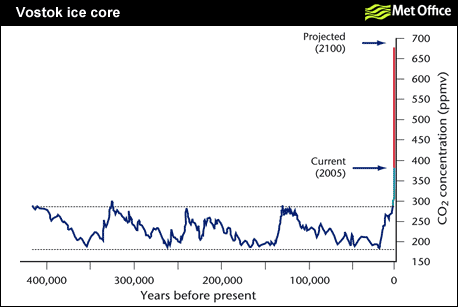
\includegraphics[width=100mm]{s2-co2increase.png}
\centering
\caption{\ce{CO2} concentrations in an ice core from Vostok, Antarctica. Source: U.K Met Office}
\label{fig:Vostok}
\end{figure}



\begin{figure}
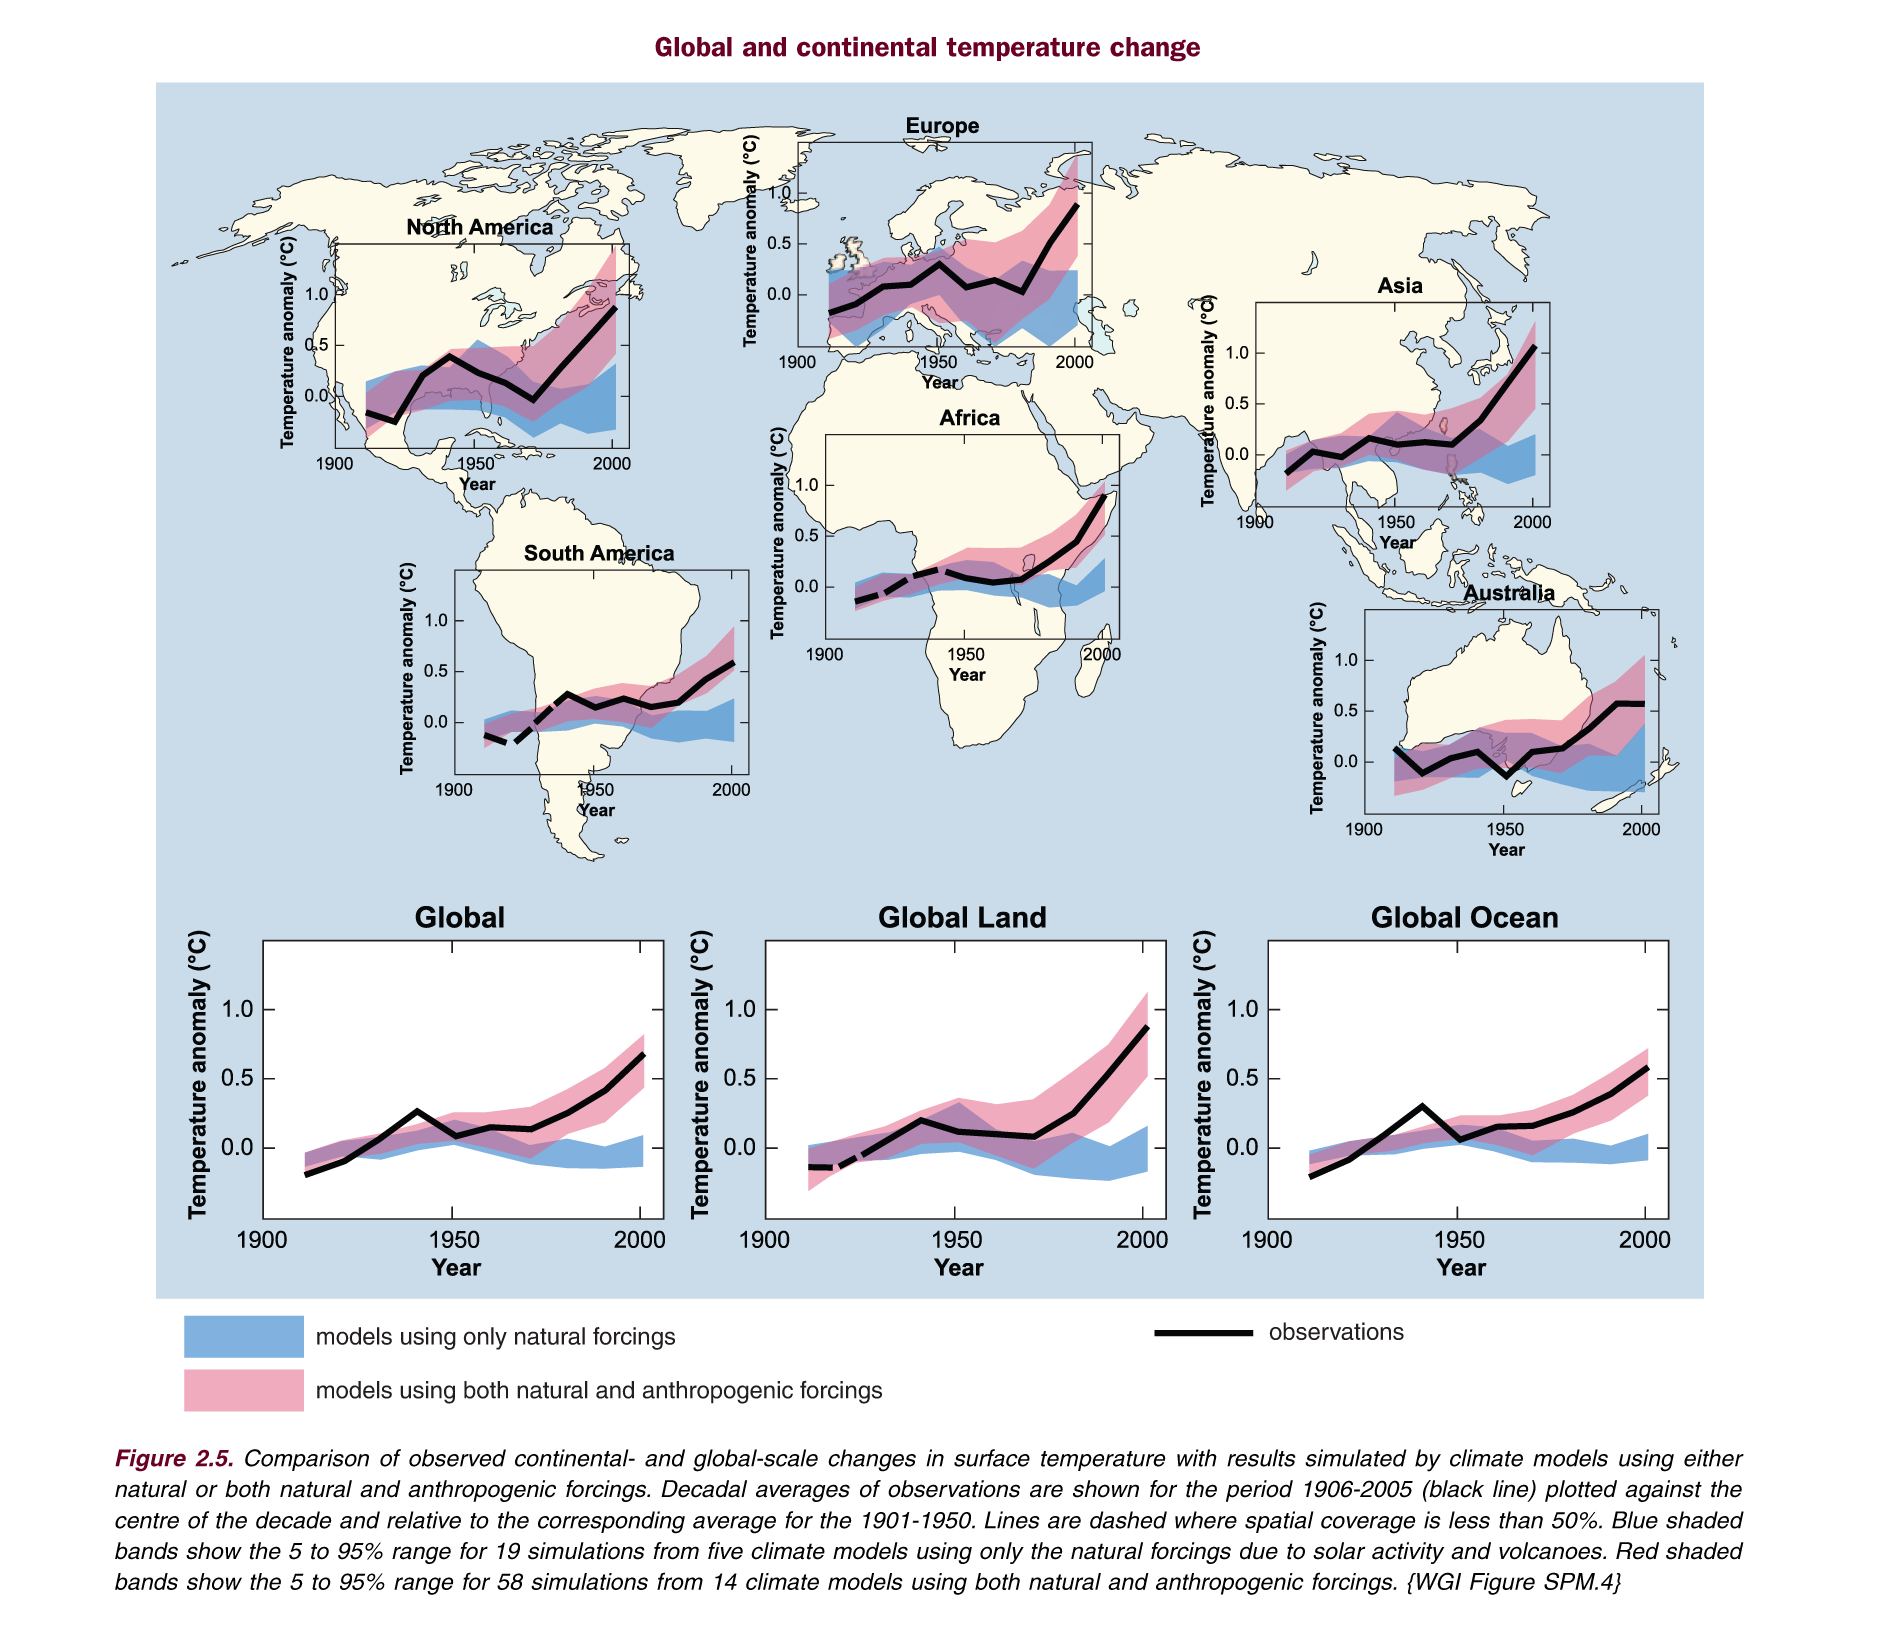
\includegraphics[width=160mm]{s2-attribution.PNG}
\centering
\caption{Global and continental temperature change. Source: IPCC 4th Assessment Report, Synthesis Report, p. 40}
\label{fig:CO2increase}
\end{figure}



Comprehensive and authoritative scientific statements on the key elements of climate change date back at least to the 1979 U.S. National Academy of Sciences report (the Charney report).\footcite[][]{Charney1979}
The report concluded that human activities --- particularly greenhouse gas emissions --- were altering the climate in potentially dangerous ways.
The science of climate change has been extensively examined by the Intergovernmental Panel on Climate Change (IPCC): a body established in 1988 by the World Meteorological Organization and the United Nations Environmental Programme to be the leading international body on the scientific, technical, and socio­economic assessment of climate change.
The four major reports of the IPCC in 1990, 1995, 2001, and 2007 have confirmed the basic conclusions of the Charney report, and elaborated considerably upon the causes and consequences of climate change.\footcite[][]{IPCC1990}\footcite[][]{IPCC1995}\footcite[][]{IPCC2001}\footcite[][]{IPCC2007}
In May 2009, the national science academies of the G8 countries plus Brazil, China, South Africa, and India released a remarkable joint statement.\footcite[][]{G8plusJointStatement}
The statement explains that: ``The need for urgent action to address climate change is now indisputable. For example, limiting global warming to 2°C would require a very rapid worldwide implementation of all currently available low carbon technologies''.
Among other things, it recommends that all governments ``adopt a long-term global goal and near-term emission reduction targets that will deliver an approximately 50\% reduction in global emissions from 1990 levels by 2050'' and ``collaborate in the implementation of low carbon and climate-resilient infrastructure and technologies, and in the implementation of innovative incentives, through the use of economic and regulatory instruments, to accelerate adoption of clean “green” technologies''.
These findings are echoed in recent research, including a 2013 article in \emph{Nature Climate Change} that emphasized how: ``[a] shift to a 2˚C pathway requires immediate significant and sustained global mitigation''.\footcite[][p. 1]{ChallengeTwoDegrees} \footcite[See also: ][]{EmissionTargetsTwoDegrees}



Several significant studies have examined the state of the scientific consensus on climate change.
In 2004, Naomi Oreskes published a paper in \emph{Science} that quantified this.
She examined the abstracts from 928 peer-reviewed papers and found that all of them either take no position on climate change or endorse the consensus position.\footcite[][p. 1686]{Oreskes2004}
She concludes:
\begin{quote}
This analysis shows that scientists publishing in the peer-reviewed literature agree with IPCC, the National Academy of Sciences, and the public statements of their professional societies. Politicians, economists, journalists, and others may have the impression of confusion, disagreement, or discord among climate scientists, but that impression is incorrect.\footcite[][p. 1686]{Oreskes2004}
\end{quote}
Oreskes' book \emph{Merchants of Doubt} elaborates on the article, discussing the strength of this consensus, while also providing details on the active campaigns of disinformation that fossil fuel companies have directed at decision-makers and the general public. \footcite[][]{MerchantsDoubt} \footcite[See also: ][]{ClimateCoverUp}
In 2010, a meta-analysis found that: ``97–98\% of the climate researchers most actively publishing in the field agree with the occurrence of anthropogenic climate change as outlined by the Intergovernmental Panel on Climate Change'' and ``the relative climate expertise and scientific prominence of the researchers unconvinced of climate change are substantially below that of the convinced researchers''.\footcite[][p. 1]{ExpertCredibility}
More recently, a study examined 11,944 climate-related abstracts from 1991 to 2011 and concluded that: ``[a]mong abstracts expressing a position on AGW, 97.1\% endorsed the consensus position that humans are causing global warming''.\footcite[][]{QuantConsensus}


Mitigating climate change is necessary in order for the university to achieve its academic mission. 
In the event that the world fails to curb greenhouse gas emissions and produces well over 2˚C of climate change, substantial damage is expected to be imposed on the global economy.
The Stern Review on the economics of climate change concluded that under a business-as-usual scenario, there is ``at least a 50\% risk of exceeding 5°C global average temperature change'' and that ``[s]uch changes would transform the physical geography of the world. A radical change in the physical geography of the world must have powerful implications for the human geography - where people live, and how they live their lives.''\footcite[][See long executive summary at: \url{http://www.hm-treasury.gov.uk/d/Executive_Summary.pdf}]{Stern2007}
Such an outcome threatens the growth prospects of the endowment and pension funds of the University of Toronto. 
It also creates additional geopolitical risks such as agricultural disruption and forced migration.



% Some of the text in the paragraph below is also in the FAQ section



James Powell, former President of Oberlin, Franklin and Marshall, and Reed College, has concluded that university trustees have a quasi-legal duty to do all they can about climate change, arguing:
\begin{quotation}
The board is supposed to make sure that the endowment allows for intergenerational equity, that the students who are going to Oberlin in 2075 get as much benefit from it as those there now. But with global warming, you’re guaranteeing a diminution of quality of life decades out.\footcite[][]{CaseForDivestment}
\end{quotation}
The emergence of a strong academic consensus about the key features of a problem does not mean that all academic work on the subject ceases.
For instance, scholarly work is still done on South African apartheid, despite the system having been dismantled.
When the university decided to divest from South Africa, it determined that a convincing body of evidence supporting that choice had been assembled.
A comparable body of evidence now exists about the causes and dangers of climate change.
Taking action to address climate change is not an example of needlessly taking sides in a controversial issue. Rather, it is a matter of taking part in a necessary global transition. 
If the world fails to constrain the worst impacts of climate change, serious deleterious impacts can be expected for Canada and the University of Toronto.



	\subsection{The University of Toronto is already taking action on climate change}
	\label{UTTakenSides}



The university has already taken a number of actions motivated by concern about climate change and a desire to reduce the university's greenhouse gas pollution impact.
The university's actions show climate change to be ``directly pertinent to higher education and academic research'', as required by the \nameref{PolicySocialPolitical}.



In November 2009, the University of Toronto signed the ``Ontario Universities Committed to a Greener World'' pledge. In part, the pledge reads:
\begin{quote}
The Ontario university community is deeply aware of the challenges that face the world arising from climate change and the degradation of natural environments. Our universities accept this special responsibility on three scores: to assist in finding solutions to the challenges of environmental sustainability; to share knowledge about sustainability and climate change; and to incorporate, wherever possible, principles of sustainability into our own operations.\footcite[][]{OntarioPledge}
\end{quote}
The decision to divest from fossil fuels stocks would be wholly in keeping with these objectives.
Redirecting investment away from fossil fuels is a key part of solving the challenge of environmental sustainability.
Furthermore, by taking the lead and choosing to divest, the University of Toronto would send an important signal about how it views the future of energy.
This is also an opportunity to incorporate sustainability into university operations in a critical way, by having the university's values reflected in its stock portfolio.



\textbf{Policies and infrastructure decisions justified with reference to climate change}
\label{UofTActions}



% This section incorporates text provided by Jessica Vogt



In 2010, the university adopted an Environmental Protection Policy.\footcite[][]{UTEnvProtectionPolicy}
The policy recognizes that ``that some of [the univeristy's] activities, because of their scale and scope, have the potential, if not managed in compliance with the university’s established standards and practices, to have significant effects on the environment''.
These activities include the investments made by U of T.
Among the principles listed, the policy says the university will:
\begin{itemize}
	\item Operate so as to minimize negative impacts on the environment,
	\item Adopt practices that reflect the conservation and wise use of natural resources, and
	\item Respect biodiversity
\end{itemize}
The policy also lists the conservation of energy and the reduction of waste as objectives.



In 2004, the university established the Sustainability Office at St. George campus and the Environmental Affairs Office at the Mississauga campus.\footcite[][]{UTSustOffice} \footcite[][]{}
The Environmental Affairs Office tracks the electricity and natural gas use of buildings in real-time, and makes the data available through their building dashboard.\footnote{See: \url{http://buildingdashboard.net/utorontom/}}
In 2007, a Sustainability Office was established at the Scarborough campus.\footcite[See: ][]{UTSustOffice}
This office explains that: ``[a] number of retrofit projects have been undertaken to reduce energy consumption as well as \ce{CO2} emissions''.\footcite[][]{UTSustOfficeEnergy}
The Facilities and Services Department provides a breakdown of the university's GHG emissions.\footnote{See: \url{http://sustain.fs.utoronto.ca/campus-footprint/}}
U of T also has a Sustainability Board, charged with providing guidance, support, and coordination of initiatives between the three campuses.



The annual reports of the Sustainability Office include data on the GHG emissions from the St. George Campus.\footcite[][]{UTSustOffice2010report}
The 2010 report partly justifies the installation of a solar hot water system at the Faculty of Physical Education and Health on the basis of reduced GHG pollution.\footcite[][p. 17]{UTSustOffice2010report}
A 2010 press release describes how paper use at the St. George campus produces ``greenhouse gas emissions of about 1,500 tonnes'' and describes how an expanded paper conservation program aims to reduce that.\footcite[][]{UTGoingGreener2010}
In a comparison of sustainability indicators, the 2011 strategic plan of the Sustainability Office lists ``[g]reenhouse gas emissions'' as an area where U of T ``leads''.\footcite[][p. 1]{UTSustOfficePlan}
In particular, it says that the office will ``[w]ork with specific university constituencies... to identify financially sound opportunities for emission reduction''.
The plan also lists ``[c]limate and [r]esources'' under ``priority long-term goals and key actions'' and identifies GHG emissions as a ``key performance indicator''.




\textbf{Academic programming}
\label{UofTAcademicProgramming}


In 2005, the university established a new Centre for Global Change Science (CGCS), which has since conducted exemplary research into climate change effects, as well as a wide array of public lectures focused around climate-related themes.\footnote{See: \url{http://www.cgcs.utoronto.ca/}}
Danny Harvey --- a Professor in the Department of Geography who is associated with the centre, is also the author of two important books describing the causes and consequences of climate change.\footcite[][]{Harvey1999a} \footcite[][]{Harvey1999b}
The CGCS has hosted a number of talks as part of its Distinguished Lecture Series including:
\begin{itemize}
	\item Successes and Challenges for Biodiversity Science: Distribution Responses to Climate Change --- James Clark, Duke University, September 18, 2012
	\item High Altitude Climate Change: The Survival Struggle of our Earth’s Alpine Glaciers --- Andrew Bush, University of Alberta, October 16, 2012 
	\item Assessing Vegetation Responses and Feedbacks to Climate Change --- John Gamon, University of Alberta, November 6, 2012
	\item Cumulative Carbon Emissions and the Climate Mitigation Challenge --- Damon Matthews, McGill University, February 5, 2013; and
	\item Trees to Tailpipes: Natural and Anthropogenic Influences on Global Atmospheric Composition --- Colette Heald Massachusetts Inst. of Technology, March 5, 2013.\footcite[][]{DistinguishedLecturer}
\end{itemize}


The Koffler Scientific Reserve at Jokers Hill is conducting research on how climate change is affecting plant species.\footcite[][]{KofflerCC}
The project is ``using artificial warming field arrays to elevate temperatures to those predicted for 2050''.



The Department of Computer Science operates a weekly seminar series: Collaborative Challenges for the Climate Change Research Community.\footnote{See: \url{http://www.cs.toronto.edu/climate/}}
Recent presentation topics have included climate models, building community resilience to climate change, the response of freshwater ecosystems in Canada's north to climate change, and low-carbon cities.



The university also offers courses on climate-change-related themes, including:
\begin{itemize}
	\item Applied Climate Change: Gaining Practical Skills for Climate Change Adaptation (UTSC Summer Institute 2013)
	\item Gaining Practical Skills for Climate Change Adaptation (UTSC Summer Institute 2013)
	\item Climate Change Law (LAW269H1S); and
	\item Climate Change and Human Health (CEM 406).
\end{itemize}
The University of Toronto also maintains an Environmental Research Database which includes ``430 University of Toronto researchers across all three U of T campuses engaged in environment-related research encompassing a wide spectrum of interests ranging from environmental finance to climate change''.\footcite[][]{UTEnvResDB}



% Material from Stuart incorporated



U of T identifies some of its own faculty as climate change experts.
As part of the university's `Boundless' campaign, Richard Peltier at the Centre for Global Change Science is identified as a ``Physicist and Climate Scientist''.\footcite[][]{PeltierBoundless}
Ron Dembo --- the founder and CEO of Zerofootprint, a software company focused on reducing humanity's environmental footprint --- is also included as one of the campaign volunteers.\footcite[][]{DemboBoundless}
On his Boundless campaign page, Professor of Public Health Sciences and of Surgery Abdallah Daar identifies climate change as a threat that ``do[es] not carry passports or recognize borders''.\footcite[][]{DaarBoundless}
The Institute of Global Health Equity and Innovation within the Faculty of Medicine lists climate change as an area of research.\footcite[][]{GlobalHealthEquity}
Along with Lorraine Sugar from the World Bank, Professor Chris Kennedy, at the Department of Civil Engineering, co-authored ``A low carbon infrastructure plan for Toronto, Canada'' in the \emph{Canadian Journal of Civil Engineering}.\footcite[][p. 86-96]{Sugar2012}
They estimate that implementation of their strategies could produce a 31\% reduction in per capita GHG emissions by 2031.



Climate change is certainly an area of active scholarly research, but that research does not question the fundamental connection between burning fossil fuels and warming the planet. 
Nor does it challenge the argument that climate change is likely to cause a great deal of social injury and human suffering.
Rather, the academic work being conducted on climate change at U of T reinforces the case for divestment.



	\subsection{Fossil fuel companies acknowledge the reality and danger of climate change}



% Ideally, this section should be read while listening to Leonard Cohen's "Everybody knows"

	

Fossil fuel companies explicitly acknowledge that climate change poses a threat to the world at large, as well as to their operations and profitability.\footcite[][]{FFcorpsPlanning} \footcite[][]{OilCosFearFI} \footcite[][]{DemiseOfCrudeDenial} \footcite[][]{DoTheOpposite}
In their 2011 submission to the Carbon Disclosure Project, ExxonMobil acknowledged ``risks to society and ecosystems from rising greenhouse gas emissions''.\footcite[][]{ExxonCDP2011}
In the same document, ExxonMobil acknowledges that climate change may alter ``risks of weather extremes'' and states that they ``manage these risks through robust design and operations contingency planning''.
Speaking at the Council on Foreign Relations on June 27th 2012, ExxonMobil CEO Rex Tillerson stated: `` So I'm not disputing that increasing \ce{CO2} emissions in the atmosphere is going to have an impact. It'll have a warming impact.''\footcite[][]{Tillerson}
On their website, ConocoPhillips recognizes that: ``human activity, including the burning of fossil fuels, is contributing to increased concentrations of greenhouse gases (GHG) in the atmosphere that can lead to adverse changes in global climate''.\footcite[][]{ConocoPhillipsCC}
They also assert that ``effective climate change policy must... [r]esult in the stabilization of global GHG atmospheric concentrations at safe levels''.
On their global website, Shell says that: ``\ce{CO2} emissions must be reduced to avoid serious climate change''.\footcite[][]{ShellClimateChange} \footnote{Shell also has a climate change advisor, with a blog at: \url{http://blogs.shell.com/climatechange/}}
Chevron's website asserts that: ``a successful climate policy will be one in which the reduction of GHGs is accomplished equitably by the top emitting countries of the world through long-term and coordinated national frameworks''.\footcite[][]{}
On BP's website, they summarize the conclusions of the Intergovernmental Panel on Climate Change and say that even with more aggressive GHG mitigation policies growth in \ce{CO2} emissions will ``probably not [be] enough to limit warming to no more than 2˚C''.\footcite[][]{BPClimateChange}
Entergy --- an S\&P 500 company with nearly 15,000 employees --- also acknowledges material risks from climate change.
Jeff Williams, director of climate consulting for Entergy, states: ``Clearly we are facing risks from sea level rise, more intense storms, flooding and surge damage''.\footcite[][]{ShiftToClimatePreparedness}


In numerous advertising campaigns, fossil fuel companies have acknowledged that climate change is taking place, and even that they bear some responsibility for dealing with it.
At the same time, much of the fossil fuel industry's advertising is misleading in its description of environmental effects.
For instance, recent advertising in Canada has misrepresented the effect of oil sands extraction on freshwater.\footcite[][]{PembinaOilAds}


\begin{vcom}
There are lots of greenwashing ads - possibly even from Shell - that we can use to demonstrate that the fossil fuel industry itself acknowledges climate change.
\end{vcom}



As elaborated in \nameref{sec:LikeTobacco} there are many parallels between fossil fuel divestment and divestment from tobacco companies.
Among these the awareness of the producers themselves that their products are harmful and dangerous.
When the University of Toronto decided to divest from tobacco companies, President David Naylor noted the significance of tobacco companies themselves acknowledging the health risks of smoking: ``that there is no serious academic or social debate about tobacco's health effects – even tobacco manufacturers by now concede them.''\footcite[][]{TStarSellOff}



% END SECTION 2 - MILAN